\documentclass[leqno]{article}
% Shared QBT/Soln pack preamble for resources.danieljsmith.org.
\usepackage{graphicx}
\usepackage{dsfont}
\usepackage{mathtools}
\usepackage{amssymb}
\usepackage{amsmath}
\usepackage{amsthm}
\usepackage{float}
\usepackage{ragged2e}
\usepackage{tensor}
\usepackage{fancyhdr}
\usepackage{empheq}
\usepackage[most]{tcolorbox}
\usepackage{enumitem}
\usepackage{dirtytalk}
\usepackage{marginnote}
\usepackage{microtype}
\usepackage[
  a4paper,
  left=0.8in,
  right=1in,
  top=1in,
  bottom=0.5in,
  headheight=14pt,
  headsep=0.4in
]{geometry}
\setlength{\parindent}{0cm}

% TikZ / PGFPlots
\usepackage{pgfplots}
\pgfplotsset{compat=1.18}
\usepgfplotslibrary{fillbetween, polar}
\usetikzlibrary{calc, positioning}
\usetikzlibrary{angles, quotes}
\usetikzlibrary{arrows.meta}
\usetikzlibrary{decorations.pathreplacing, decorations.markings}
\usetikzlibrary{patterns}
\usetikzlibrary{intersections}

% Links and contents
\usepackage[colorlinks=true,linkcolor=black,citecolor=magenta,urlcolor=black]{hyperref}%
\urlstyle{same}

% Pack macros
\RenewDocumentCommand{\marks}{o m}{%
  \IfValueTF{#1}%
    {\marginnote{\raggedright\textbf{[#2]}}[#1]}%
    {\marginnote{\raggedright\textbf{[#2]}}}%
}

\newcommand{\vspacerule}[2]{%
  \par\vspace*{#1}%
  \noindent\hrulefill\par
  \vspace*{#2}%
}

\definecolor{scarlet}{RGB}{205, 40, 75}

% Worked-solution box, adapted from the TMUA worked-solutions box. A white breakable box with a left scarlet rule and no surrounding
% frame or tint. A part that breaks fills the rest of its page, so the rule
% runs to the bottom margin; the unbroken or last part ends in a short
% horizontal foot rule so a solution visibly stops. Unlike the TMUA box there
% is no answer label and no extra \parskip: these solutions mix \\ line breaks
% with blank lines, so paragraph skips would make the spacing uneven. The box
% does not grow to the left, so the rule sits at the text edge; growing to the
% right keeps the usable line width close to the old tcolorbox Solution box.
\newtcolorbox{djsSolution}{%
  enhanced, breakable, frame hidden, sharp corners, colback=white,
  height fixed for=first and middle, height fill,
  extras unbroken and last={natural height},
  borderline west={2.2pt}{0pt}{scarlet},
  left=11pt, right=0pt, top=5pt, bottom=13pt,
  before skip=13pt, after skip=4pt,
  grow to right by=10mm,
  overlay unbroken and last={%
    \fill[scarlet] (frame.south west)
      rectangle ([xshift=3.5cm, yshift=2.2pt]frame.south west);},
  before upper={{\color{scarlet}\bfseries Solution}\par\vspace{4pt}}}

% Optional smaller figure inside a solution box. \scalebox shrinks node text
% with the drawing. Not applied to existing figures.
\newcommand{\SolnFigureScale}{0.85}
\newsavebox{\djsSolnFigureBox}
\newenvironment{djsSolutionFigure}
  {\par\vspace{4pt}\begin{center}\begin{lrbox}{\djsSolnFigureBox}}
  {\end{lrbox}\scalebox{\SolnFigureScale}{\usebox{\djsSolnFigureBox}}%
   \end{center}\vspace{2pt}\par}

\newcommand{\cxl}[2]{%
  \tikz[baseline=(X.base)]{%
    \node[inner sep=0pt, outer sep=0pt, text=#1] (X) {$#2$};
    \draw[#1, line width=0.4pt] (X.south west)--(X.north east);
  }%
}

% Page-style hook run at the contents page and each question's opening page.
% A no-op for QBT packs; \djsSolnHeader points it at the fancy header.
\newcommand{\djsQuestionPageStyle}{}

\newcommand{\questionitem}{%
  \djsQuestionPageStyle
  \item\phantomsection
  \addcontentsline{toc}{section}{Question \number\value{enumi}}%
}

\renewcommand{\contentsname}{Questions}

\newcommand{\djsPackHeader}[1]{%
  \pagestyle{fancy}%
  \fancyhead{}%
  \fancyfoot{}%
  \renewcommand{\headrulewidth}{0.9pt}%
  \lhead{#1}%
  \chead{}%
  \rhead{\href{https://danieljsmith.org}{danieljsmith.org}}%
}

\newcommand{\djsQbtHeader}[1]{%
  \djsPackHeader{#1}%
}

% Solutions packs show the header only on the contents page and each
% question's opening page, so it never appears part-way through a solution.
% \thispagestyle marks the next page shipped out, which is the question's
% page because every solution question starts after a \newpage.
\newcommand{\djsSolnHeader}[1]{%
  \djsPackHeader{\textit{Solutions} - #1}%
  \pagestyle{empty}%
  \renewcommand{\djsQuestionPageStyle}{\thispagestyle{fancy}}%
}

\newcommand{\djsFrontMatter}{%
  \djsQuestionPageStyle
  \vspace*{20pt}%
  \tableofcontents
  \newpage
}


\djsQbtHeader{Elastic Potential Energy}

\begin{document}
\djsFrontMatter
\begin{enumerate}[
  label=\textbf{\arabic*.},
  leftmargin=*,
  topsep=0pt,
  partopsep=0pt,
  parsep=0pt
]

% ---- Question 1 ----
\questionitem
% [Source: _QBT__Elastic_Potential_Energy, Q1]

One end of a light elastic string, of natural length $2a$ and modulus of elasticity $2mg$, is attached to a fixed point $O$. The other end of the string is attached to a particle $P$ of mass $m$. The string is vertical with $P$ directly above $O$. The particle $P$ is pulled vertically upwards until the extension of the string is $2a$. The particle $P$ is then released from rest. \\
\begin{enumerate}[label=\textbf{(\alph*)}]
  \item Find the speed of $P$ when it is at a distance $\dfrac{3}{2}a$ above $O$. \marks{3} \\
  \item Find the initial acceleration of $P$ when it is released from rest. \marks{2} \\
\end{enumerate}

\newpage

% ---- Question 2 ----
\questionitem
% [Source: _QBT__Elastic_Potential_Energy, Q2]

A light elastic string has natural length $2.5$ metres and modulus of elasticity $15$ newtons. \\

One end of the elastic string is attached to a particle of mass $0.75\,\mathrm{kg}$. \\

The other end of the elastic string is attached to a fixed point $O$. \\

The particle is released from rest at a point $A$, which is $2.9$ metres vertically below $O$. \\

\begin{enumerate}[label=\textbf{(\alph*)}]
  \item Calculate the elastic potential energy stored in the string when the particle is at $A$. \marks{2} \\
  \item The point $B$ is $4.0$ metres vertically below $O$. \\
  Calculate the gravitational potential energy lost by the particle as it moves from $A$ to $B$. \marks{2} \\
  \item Find the speed of the particle at $B$. \marks{3} \\
  \item The point $C$ is $3.3$ metres vertically below $O$. \\
  Explain, showing any calculations that you make, why the speed of the particle is increasing the first time that the particle is at $C$. \marks{3} \\
\end{enumerate}

\newpage

% ---- Question 3 ----
\questionitem
% [Source: _QBT__Elastic_Potential_Energy, Q3]

A particle $P$ of mass $m$ is attached to one end of a light elastic string of natural length $a$ and modulus $2mg$. The other end of the string is attached to a fixed point $O$ on a rough plane inclined at $30^\circ$ to the horizontal. \\

The string lies along a line of greatest slope, with $O$ below $P$. The particle is initially at rest on the plane with the string at its natural length. \\

The coefficient of friction between $P$ and the plane is $\dfrac{1}{\sqrt{3}}$. \\

The particle is projected up the plane, away from $O$, with speed $\sqrt{\dfrac{3ga}{2}}$. \\

Find the greatest extension of the string during the subsequent motion. \marks{5} \\

\newpage

% ---- Question 4 ----
\questionitem
% [Source: _QBT__Elastic_Potential_Energy, Q4]

The points $A$ and $B$ are at the same horizontal level and are $24a$ apart. The ends of a light elastic string, of natural length $18a$ and modulus of elasticity $\lambda$, are attached to $A$ and $B$. A particle $P$ of mass $m$ is attached to the midpoint of the string. The system is in equilibrium with $P$ at a distance $5a$ below $M$, the midpoint of $AB$. \\
\begin{enumerate}[label=\textbf{(\alph*)}]
  \item Find $\lambda$ in terms of $m$ and $g$. \marks{3} \\
\end{enumerate}
The particle $P$ is pulled down vertically and released from rest from a position $9a$ below $M$. \\
\begin{enumerate}[label=\textbf{(\alph*)}, resume]
  \item Find, in terms of $a$ and $g$, the speed of $P$ as it passes through its equilibrium position. \marks{4} \\
\end{enumerate}

\newpage

% ---- Question 5 ----
\questionitem
% [Source: _QBT__Elastic_Potential_Energy, Q5]

A light elastic string has natural length $3a$ and modulus of elasticity $9mg$. \\
One end of the string is attached to a fixed point $O$. A particle $P$ of mass $m$ is attached to the other end. \\
The particle hangs freely in equilibrium at the point $E$, vertically below $O$. \\
\begin{enumerate}[label=\textbf{(\alph*)}]
  \item Find the length $OE$. \marks{4} \\
\end{enumerate}
The particle is then pulled vertically downwards from $E$ to a point $A$, where $OA = \dfrac{16a}{3}$, and released from rest. \\
The resistance to the motion of $P$ is a constant force of magnitude $\dfrac{1}{4}mg$. \\
\begin{enumerate}[label=\textbf{(\alph*)}, resume]
  \item Find, in terms of $a$ and $g$, the speed of $P$ as it passes through $E$. \marks{7} \\
\end{enumerate}
The particle is now held at $O$ and released from rest. \\
The resistance to the motion of $P$ is again a constant force of magnitude $\dfrac{1}{4}mg$. \\
The speed of $P$ is greatest when it is at the point $B$. \\
\begin{enumerate}[label=\textbf{(\alph*)}, resume]
  \item Find the distance $OB$. \marks{4} \\
\end{enumerate}

\newpage

% ---- Question 6 ----
\questionitem
% [Source: _QBT__Elastic_Potential_Energy, Q6]

\begin{figure}[H]
    \centering
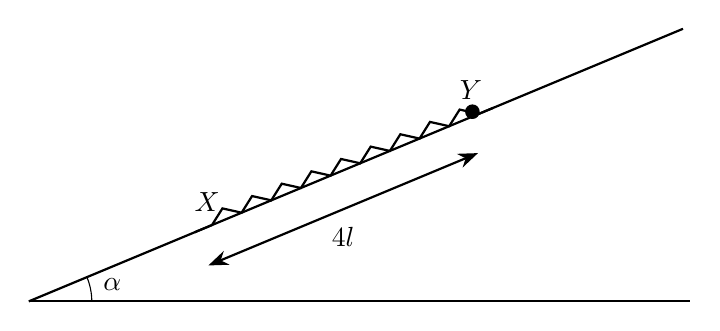
\begin{tikzpicture}[scale=1.2]
\pgfmathsetmacro{\ang}{atan(5/12)}
\def\planeLen{7.5}
\def\xstart{1.9}
\def\lead{0.20}
\def\seg{0.17}
\pgfmathsetmacro{\springLen}{\lead + 17*\seg}
\def\amp{0.12}
\def\measureOff{0.38}

\coordinate (A) at (0,0);
\coordinate (H) at (7.0,0);
\coordinate (Top) at (\ang:\planeLen);
\coordinate (X) at ($(A)+(\ang:\xstart)$);
\coordinate (Y) at ($(X)+(\ang:\springLen)$);
\coordinate (Xm) at ($(X)+(\ang-90:\measureOff)$);
\coordinate (Ym) at ($(Y)+(\ang-90:\measureOff)$);

\draw[thick] (A) -- (H);
\draw[thick] (A) -- (Top);

\begin{scope}[shift={(X)}, rotate=\ang]
  \draw[thick]
    (0,0) -- (\lead,0)
    \foreach \k in {1,...,9} {
      -- ++(\seg,\amp)
      -- ++(\seg,-\amp)
    }
    -- ++(\seg,0);
\end{scope}

\fill[black] ([yshift=2.5pt, xshift=2.5pt]Y) circle (2.2pt);

\draw[{Stealth[length=2.5mm]}-{Stealth[length=2.5mm]}, thick] (Xm) -- (Ym)
  node[midway, below=5pt, fill=white, inner sep=1pt] {$4l$};

\pic["$\alpha$", draw, angle radius=8mm, angle eccentricity=1.35]
  {angle=H--A--Top};

\node[above right, yshift=4pt, xshift=-3.5pt] at (X) {$X$};
\node[above, yshift=4pt, xshift=2.5pt] at (Y) {$Y$};
\end{tikzpicture}
\end{figure}


A light elastic spring has natural length $2l$ and modulus of elasticity $mg$. One end of the spring is attached to a fixed point $X$ on a rough inclined plane. The other end is attached to a package $P$ of mass $m$. \\

The plane is inclined to the horizontal at an angle $\alpha$ where
\[
\tan \alpha = \dfrac{5}{12}
\] 
The package is initially held at the point $Y$ on the plane, where $XY = 4l$. The point $Y$ is higher than $X$ and $XY$ is a line of greatest slope of the plane, as shown. The package is released from rest at $Y$ and moves down the plane. \\

The coefficient of friction between $P$ and the plane is $\dfrac{1}{4}$. \\

By modelling $P$ as a particle, \\
\begin{enumerate}[label=\textbf{(\alph*)}]
  \item show that the acceleration of $P$ at the instant when it is released is
  \[
  \dfrac{15}{13}g
  \]
  down the plane. \marks{5} \\
  \item find, in terms of $g$ and $l$, the speed of $P$ at the instant when the spring first regains its natural length. \marks{6} 
\end{enumerate}

\newpage

% ---- Question 7 ----
\questionitem
% [Source: _QBT__Elastic_Potential_Energy, Q7]

\begin{figure}[H]
    \centering
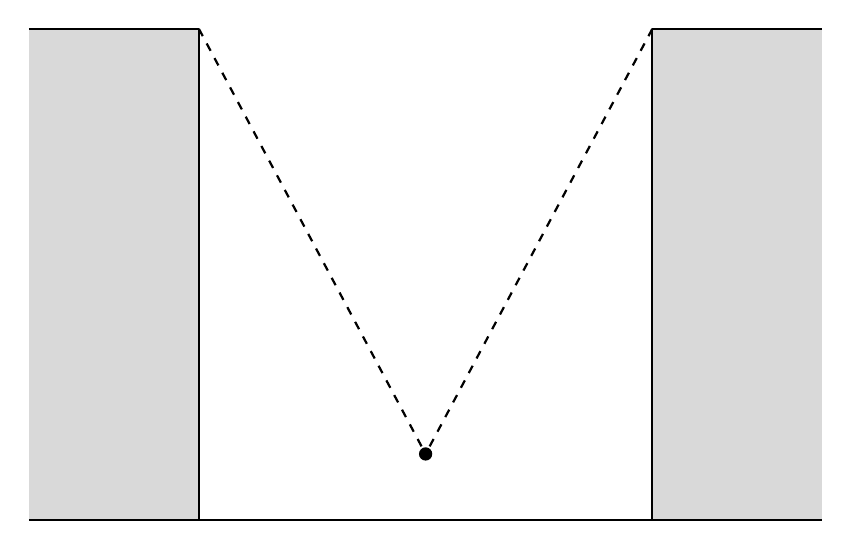
\begin{tikzpicture}[scale=0.12]
\def\depth{52}
\def\halfwidth{24}
\def\outer{42}
\def\starth{7}

\coordinate (Ltop) at (-\halfwidth,\depth);
\coordinate (Rtop) at (\halfwidth,\depth);
\coordinate (Lbase) at (-\halfwidth,0);
\coordinate (Rbase) at (\halfwidth,0);
\coordinate (H) at (0,\starth);

\fill[gray!30] (-\outer,0) rectangle (-\halfwidth,\depth);
\fill[gray!30] (\halfwidth,0) rectangle (\outer,\depth);

\draw[thick] (-\outer,\depth) -- (-\halfwidth,\depth);
\draw[thick] (\halfwidth,\depth) -- (\outer,\depth);
\draw[thick] (-\outer,0) -- (-\halfwidth,0);
\draw[thick] (\halfwidth,0) -- (\outer,0);
\draw[thick] (Ltop) -- (Lbase);
\draw[thick] (Rtop) -- (Rbase);
\draw[thick] (Lbase) -- (Rbase);

\draw[dashed, thick] (Ltop) -- (H);
\draw[dashed, thick] (Rtop) -- (H);
\fill[black] (H) circle (20pt);
\end{tikzpicture}
\end{figure}


A stunt performer is attached to two identical light elastic cords. One end of each cord is fixed to opposite sides of the rim of a vertical shaft, as shown in the diagram above. \\

The performer has mass $80\,\mathrm{kg}$ and is modelled as a particle. Initially the performer is held at rest at the centre of the shaft, $7$ metres above the floor. The shaft is $52$ metres deep and $48$ metres wide. Each elastic cord has natural length $30$ metres and modulus of elasticity $3150\,\mathrm{N}$. \\

The performer is released from rest. \\

\begin{enumerate}[label=\textbf{(\alph*)}]
  \item Show that the speed of the performer when the cords first become slack is $25\,\mathrm{m\,s^{-1}}$ correct to two significant figures. \marks{6} \\
  \item Determine whether the performer is moving up or down when the cords become taut again. \marks{5} \\
\end{enumerate}

\newpage

% ---- Question 8 ----
\questionitem
% [Source: _QBT__Elastic_Potential_Energy, Q8]

A spring of natural length $a$ is suspended from a fixed point $A$. A package $P$ of mass $m$ is attached to the lower end of the spring. \\

The package is initially at the point $B$, vertically below $A$, where $AB=a$. \\

The package is projected vertically downwards from $B$ with speed $\sqrt{ag}$. \\

It first comes to instantaneous rest at the point $C$, where $AC=2a$. \\

Air resistance is modelled as negligible. By modelling the spring as light and modelling $P$ as a particle, \\
\begin{enumerate}[label=\textbf{(\alph*)}]
  \item show that the modulus of elasticity of the spring is $3mg$ \marks{5} \\
  \item
  \begin{enumerate}[label=(\roman*)]
    \item Show that $P$ attains its maximum speed when the extension of the spring is $\dfrac{1}{3}a$ \marks{2}
    \item Hence find the maximum speed, giving your answer in terms of $a$ and $g$. \marks{4} \\
  \end{enumerate}
  \item In reality, the spring is not light. \\
  State one way in which this would affect your energy equation in part (b). \marks{1} \\
\end{enumerate}

\newpage

% ---- Question 9 ----
\questionitem
% [Source: _QBT__Elastic_Potential_Energy, Q9]

A light elastic string with natural length $l$ and modulus of elasticity $kmg$ has one end attached to a fixed point $A$ on a rough inclined plane. The other end of the string is attached to a package of mass $m$. \\
The plane is inclined at an angle $\theta$ to the horizontal, where
\[
\tan \theta = \dfrac{3}{4}
\] \\
The package is initially held at the point $C$ on a line of greatest slope of the plane below $A$, where $AC = 3l$. The package is then projected down the plane with speed $2\sqrt{gl}$ and first comes to rest at the point $B$, where $AB = 5l$. \\
The coefficient of friction between the package and the plane is $\dfrac{1}{2}$. \\
By modelling the package as a particle, \\
\begin{enumerate}[label=\textbf{(\alph*)}]
  \item show that
  \[
  k = \dfrac{2}{5}
  \]
  \marks[-20pt]{6}
  \item find the acceleration of the package at the instant it starts to move back up the plane from the point $B$. \marks{5} \\
\end{enumerate}

\newpage


% ---- Question 10 ----
\questionitem
% [Source: _QBT__Elastic_Potential_Energy, Q10]

\begin{figure}[H]
    \centering
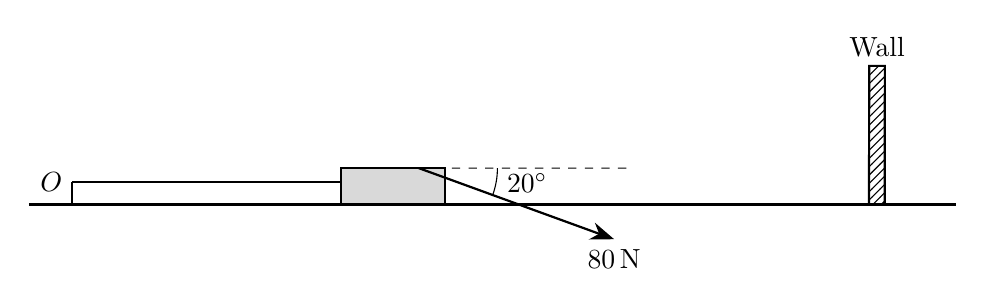
\begin{tikzpicture}[scale=1.1]
\def\surfL{-0.5}
\def\surfR{10.2}
\def\wallx{9.2}
\def\wallw{0.18}
\def\wallh{1.6}
\def\anchory{0.26}
\def\blockx{3.1}
\def\bw{1.2}
\def\bh{0.42}
\def\forceang{-20}
\def\forcelen{2.4}
\def\reflen{2.4}

\coordinate (S0) at (\surfL,0);
\coordinate (S1) at (\surfR,0);
\coordinate (A0) at (0,0);
\coordinate (O) at (0,\anchory);
\coordinate (BL) at (\blockx,0);
\coordinate (BR) at ($(BL)+(\bw,0)$);
\coordinate (TL) at ($(BL)+(0,\bh)$);
\coordinate (TR) at ($(BR)+(0,\bh)$);
\coordinate (Attach) at ($(BL)+(0,\anchory)$);
\coordinate (P) at ($(TL)!0.75!(TR)$);
\coordinate (H) at ($(P)+(\reflen,0)$);
\coordinate (F) at ($(P)+(\forceang:\forcelen)$);
\coordinate (WBL) at (\wallx,0);
\coordinate (WBR) at ($(WBL)+(\wallw,0)$);
\coordinate (WTL) at ($(WBL)+(0,\wallh)$);
\coordinate (WTR) at ($(WBR)+(0,\wallh)$);

\draw[thick] (S0) -- (S1);
\draw[thick] (A0) -- (O);
\draw[thick] (O) -- (Attach);
\draw[thick, fill=gray!30] (BL) rectangle (TR);

\fill[pattern=north east lines] (WBL) rectangle (WTR);
\draw[thick] (WBL) -- (WTL) -- (WTR) -- (WBR);

\draw[dashed] (P) -- (H);
\draw[-{Stealth[length=3mm]}, thick] (P) -- (F) node[below] {$80\,\mathrm{N}$};
\pic["$20^\circ$" {yshift=1.5pt}, draw, angle radius=10mm, angle eccentricity=1.4]
  {angle=F--P--H};

\node[left] at (O) {$O$};
\node[above] at ($(WTL)!0.5!(WTR)$) {Wall};
\end{tikzpicture}
\end{figure}


A block of mass $6\,\mathrm{kg}$ rests on a rough horizontal surface and is attached to a fixed point $O$ by a light elastic string. Initially the block is at rest $2.4\,\mathrm{m}$ from $O$. \\

The elastic string has natural length $2\,\mathrm{m}$ and modulus of elasticity $80\,\mathrm{N}$. \\

The coefficient of friction between the block and the surface is $0.25$. \\
A force of magnitude $80\,\mathrm{N}$ is applied to the block towards a vertical wall. The force acts at an angle of $20^\circ$ below the horizontal, as shown in the diagram. \\

The block moves in a straight line perpendicular to the wall, and the wall is sufficiently far away that the block does not reach it during the motion considered. \\
\begin{enumerate}[label=\textbf{(\alph*)}]
  \item Show that the block has moved $0.94\,\mathrm{m}$, correct to 2 significant figures, when the forces acting on it are in equilibrium. \marks{4} \\
  \item State one limitation of the model. \marks{1} \\
  \item Find the maximum speed of the block. \marks{4} \\
\end{enumerate}

\end{enumerate}
\end{document}
